\section{Implementing the Mixture of Gaussians VAE (GMVAE)}

Recall that in Problem \ref{p1}, the VAE’s prior distribution was a parameter-free isotropic Gaussian $p(\bz) = \calN(\bz \mid 0,I)$. 
While this original setup works well, there are settings in which we desire more expressivity to better model our data. In this 
problem we will implement the GMVAE, which has a mixture of Gaussians as the prior distribution. Specifically:

\begin{equation} \label{eq:7}
    p_{\theta}(\bz) = \sum\limits_{i=1}^{k} \frac{1}{k} \calN\left(\bz \mid \mu_i, \text{diag}\left(\sigma_i^2\right)\right)
\end{equation}

where $i \in \{1,...,k\}$ denotes the $i^{\text{th}}$ cluster index. For notational simplicity, we shall subsume our mixture of 
Guassian parameters ${\{\mu_i, \sigma_i\}}_{i=1}^{k}$ into our generative model parameters $\theta$. For simplicity, we have also 
assumed fixed uniform weights $1/k$ over the possible different clusters. Apart from the prior, the GMVAE shares an identical setup 
as the VAE:

\begin{equation} \label{eq:8}
    q_{\phi}(\bz \mid \bx) = \calN\left(\bz \mid \mu_{\phi}\left(\bx\right), \text{diag}\left(\sigma_{\phi}^2\left(\bx\right)\right)\right)
\end{equation}

\begin{equation} \label{eq:9}
    p_{\theta}(\bx \mid \bz) = \text{Bern}\left(\bx \mid f_{\theta}\left(\bz\right)\right)
\end{equation}

Although the ELBO for the GMVAE: $\E_{q_{\phi}(\bz)}[\log p_{\theta}(\bx \mid \bz)] - \KL(q_{\phi}(\bz \mid \bx) \mid\mid p_{\theta}(\bz))$ is identical to 
that of the VAE, we note that the KL term $\KL(q_{\phi}(\bz \mid \bx) \mid\mid p_{\theta}(\bz))$ cannot be computed analytically 
between a Gaussian distribution $q_{\phi}(\bz \mid \bx)$ and a mixture of Gaussians $p_{\theta}(\bz)$. However, we can obtain its 
unbiased estimator via Monte Carlo sampling:

\begin{equation} \label{eq:10}
    \KL(q_{\phi}(\bz \mid \bx) \mid\mid p_{\theta}(\bz)) \approx \log q_{\theta}(\bz^{(1)} \mid \bx) - \log p_{\theta}(\bz^{(1)})
\end{equation}
\begin{equation} \label{eq:11}
    = \underbrace{\log \calN(\bz^{(1)} \mid \mu_{\phi}(\bx), \text{diag}(\sigma_{\phi}^2(\bx)))}_\text{\texttt{log\_normal}} - \underbrace{\log\sum\limits_{i=1}^{k} \frac{1}{k}\calN(\bz^{(1)}\mid\mu_i,\text{diag}(\sigma_i^2))}_\text{\texttt{log\_normal\_mixture}}
\end{equation}

where $\bz^{(1)} \sim q_{\phi}(\bz \mid \bx)$ denotes a single sample.

\begin{enumerate}[label=(\alph*)]
    \item \points{2a} Implement the (1) \texttt{log\_normal} and (2) \texttt{log\_normal\_mixture\_functions} in \texttt{utils.py}, and the 

    function \texttt{negative\_elbo\_bound} in \texttt{gmvae.py}. The function \texttt{log\_mean\_exp} in \texttt{utils.py} 
    will be helpful for this problem in ensuring that your implementation is numerically stable.

    \clearpage

    \item \points{2a} To train the GMVAE, run 
    \begin{verbatim}
        python main.py --model gmvae --train
    \end{verbatim}
    
    To use GPU acceleration run the command below.
    \begin{verbatim}
        python main.py --model gmvae --train --device gpu
    \end{verbatim}
    
    Once the run is complete (20000 iterations), it will output: the average (1) negative ELBO, (2) KL term, and (3) reconstruction loss as 
    evaluated on a test subset that we have selected. These three numbers will be reported to \texttt{submission/GMVAE.pkl}. To check the accuracy 
    of your values run

    \begin{verbatim}
        python grader.py 2b-0-basic
    \end{verbatim}
    
    Since we’re using stochastic optimization, you may wish to run the model multiple times and report each metric’s mean
    and the corresponding standard error. 
    
    \textbf{Hint}: the negative ELBO on the test subset should be somewhere around 97-99. If you generate other NELBO values outside this range, please
    revisit your implementation of functions in \texttt{utils.py}, specifically \texttt{sample\_gaussian}.

    Also, to visualize 200 digits sampled from $p_{\theta}(\bx)$, you can run after training: 
    \begin{verbatim}
        python main.py --model gmvae
    \end{verbatim}
    
    Your samples will be saved to: \texttt{model=gmvae\_z=10\_run=0000.png}. The generated samples should look like the image below:

    \begin{figure}[h]
        \centering
        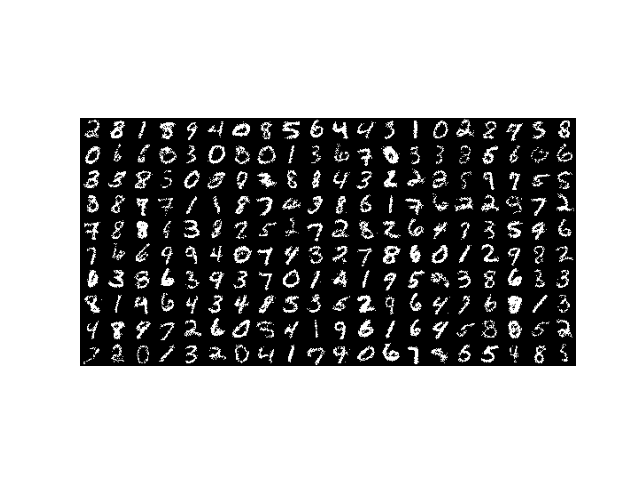
\includegraphics[width=0.8\textwidth]{./figures/gmvae_gen}
    \end{figure}

\end{enumerate}